\documentclass[UTF8,12pt]{ctexart}
\usepackage[a4paper,margin=24mm]{geometry}
\usepackage{amsmath,amssymb,bm,graphicx,adjustbox}
\newcommand{\fitmath}[1]{\begin{adjustbox}{max width=\linewidth}$\displaystyle #1$\end{adjustbox}}
\setlength{\parindent}{0pt}
\setlength{\parskip}{.7em}
\sloppy
\allowdisplaybreaks
\begin{document}
\section*{1987 年考研数学三 · 真题}
\subsection*{1987年全国硕士研究生招生考试试题}

【编者注】1987年到1996年的数学试卷IV、V均为现在的数学三。


\subsection*{（试卷IV）}

\subsection*{一、判断题（本题共5小题，每小题2分，满分10分）}

（1）\(\displaystyle \lim_{x\to0}e^{1/x}=\infty\)。


（2）\(\displaystyle \int_{-\pi}^{\pi}x^4\sin x\,dx=0\)。


（3）若级数 \(\displaystyle \sum_{n=1}^{\infty}a_n\) 与 \(\displaystyle \sum_{n=1}^{\infty}b_n\) 均发散，则级数 \(\displaystyle \sum_{n=1}^{\infty}(a_n+b_n)\) 必发散。


（4）假设 \(\displaystyle D\) 是矩阵 \(\displaystyle A\) 的 \(\displaystyle r\) 阶子式，且 \(\displaystyle D\ne0\)，但含 \(\displaystyle D\) 的一切 \(\displaystyle r+1\) 阶子式都等于0，那么矩阵 \(\displaystyle A\) 的一切 \(\displaystyle r+1\) 阶子式都等于0。


（5）连续型随机变量取任何给定实数值的概率均为零。


\subsection*{二、选择题（本大题共5小题，每小题2分，满分10分）}

（1）下列函数在其定义域内连续的是（　　）


（A）\(\displaystyle f(x)=\ln x+\sin x\)。 （B）\(\displaystyle f(x)=\begin{cases}\sin x,\allowbreak &x\le0,\allowbreak \\\cos x,\allowbreak &x>0.\end{cases}\) （C）\(\displaystyle f(x)=\begin{cases}x+1,\allowbreak &x<0,\allowbreak \\0,\allowbreak &x=0,\allowbreak \\x-1,\allowbreak &x>0.\end{cases}\) （D）\(\displaystyle f(x)=\begin{cases}\dfrac{\displaystyle 1}{\displaystyle \sqrt{|x|}},\allowbreak &x\ne0,\allowbreak \\0,\allowbreak &x=0.\end{cases}\)


（2）若 \(\displaystyle f(x)\) 在 \(\displaystyle (a,\allowbreak b)\) 内可导且 \(\displaystyle a<x_1<x_2<b\)，则至少存在一点 \(\displaystyle \xi\)，使得（　　）


（A）\(\displaystyle f(b)-f(a)=f\prime(\xi)(b-a)\;(a<\xi<b)\)。 （B）\(\displaystyle f(b)-f(x_1)=f\prime(\xi)(b-x_1)\;(x_1<\xi<b)\)。 （C）\(\displaystyle f(x_2)-f(x_1)=f\prime(\xi)(x_2-x_1)\;(x_1<\xi<x_2)\)。 （D）\(\displaystyle f(x_2)-f(a)=f\prime(\xi)(x_2-a)\;(a<\xi<x_2)\)。


（3）下列广义积分收敛的是（　　）


（A）\(\displaystyle \int_e^{+\infty}\dfrac{\displaystyle \ln x}{\displaystyle x}\,dx\)。 （B）\(\displaystyle \int_e^{+\infty}\dfrac{\displaystyle 1}{\displaystyle x\ln x}\,dx\)。 （C）\(\displaystyle \int_e^{+\infty}\dfrac{\displaystyle 1}{\displaystyle x(\ln x)^2}\,dx\)。 （D）\(\displaystyle \int_e^{+\infty}\dfrac{\displaystyle 1}{\displaystyle x\sqrt{\ln x}}\,dx\)。


（4）设 \(\displaystyle n\) 阶方阵 \(\displaystyle A\) 的秩 \(\displaystyle r(A)=r<n\)，那么在 \(\displaystyle A\) 的 \(\displaystyle n\) 个行向量中（　　）


（A）必有 \(\displaystyle r\) 个行向量线性无关。 （B）任意 \(\displaystyle r\) 个行向量都线性无关。 （C）任意 \(\displaystyle r\) 个行向量都构成极大线性无关向量组。 （D）任意一个行向量都可以由其他 \(\displaystyle r\) 个行向量线性表示。


（5）若两事件 \(\displaystyle A\) 和 \(\displaystyle B\) 同时出现的概率 \(\displaystyle P(AB)=0\)，则（　　）


（A）\(\displaystyle A\) 和 \(\displaystyle B\) 不相容（互斥）。 （B）\(\displaystyle AB\) 是不可能事件。 （C）\(\displaystyle AB\) 未必是不可能事件。 （D）\(\displaystyle P(A)=0\) 或 \(\displaystyle P(B)=0\)。


\subsection*{三、计算下列各题（每小题4分，满分16分）}

（1）求极限 \(\displaystyle \lim_{x\to0}(1+xe^x)^{1/x}\)。


（2）设 \(\displaystyle y=\ln\dfrac{\displaystyle \sqrt{1+x^2}-1}{\displaystyle \sqrt{1+x^2}+1}\)，求 \(\displaystyle y\prime\)。


（3）设 \(\displaystyle z=\arctan\dfrac{\displaystyle x+y}{\displaystyle x-y}\)，求 \(\displaystyle dz\)。


（4）求不定积分 \(\displaystyle \int e^{\sqrt{2x-1}}\,dx\)。


\subsection*{四、（本题满分10分）}

考虑函数 \(\displaystyle y=\sin x,\allowbreak \ 0\le x\le\dfrac{\displaystyle \pi}{\displaystyle 2}\)。问：


（1）\(\displaystyle t\) 取何值时，右图中阴影部分的面积 \(\displaystyle S_1\) 与 \(\displaystyle S_2\) 之和 \(\displaystyle S=S_1+S_2\) 最小？


（2）\(\displaystyle t\) 取何值时，面积 \(\displaystyle S=S_1+S_2\) 最大？


\begin{center}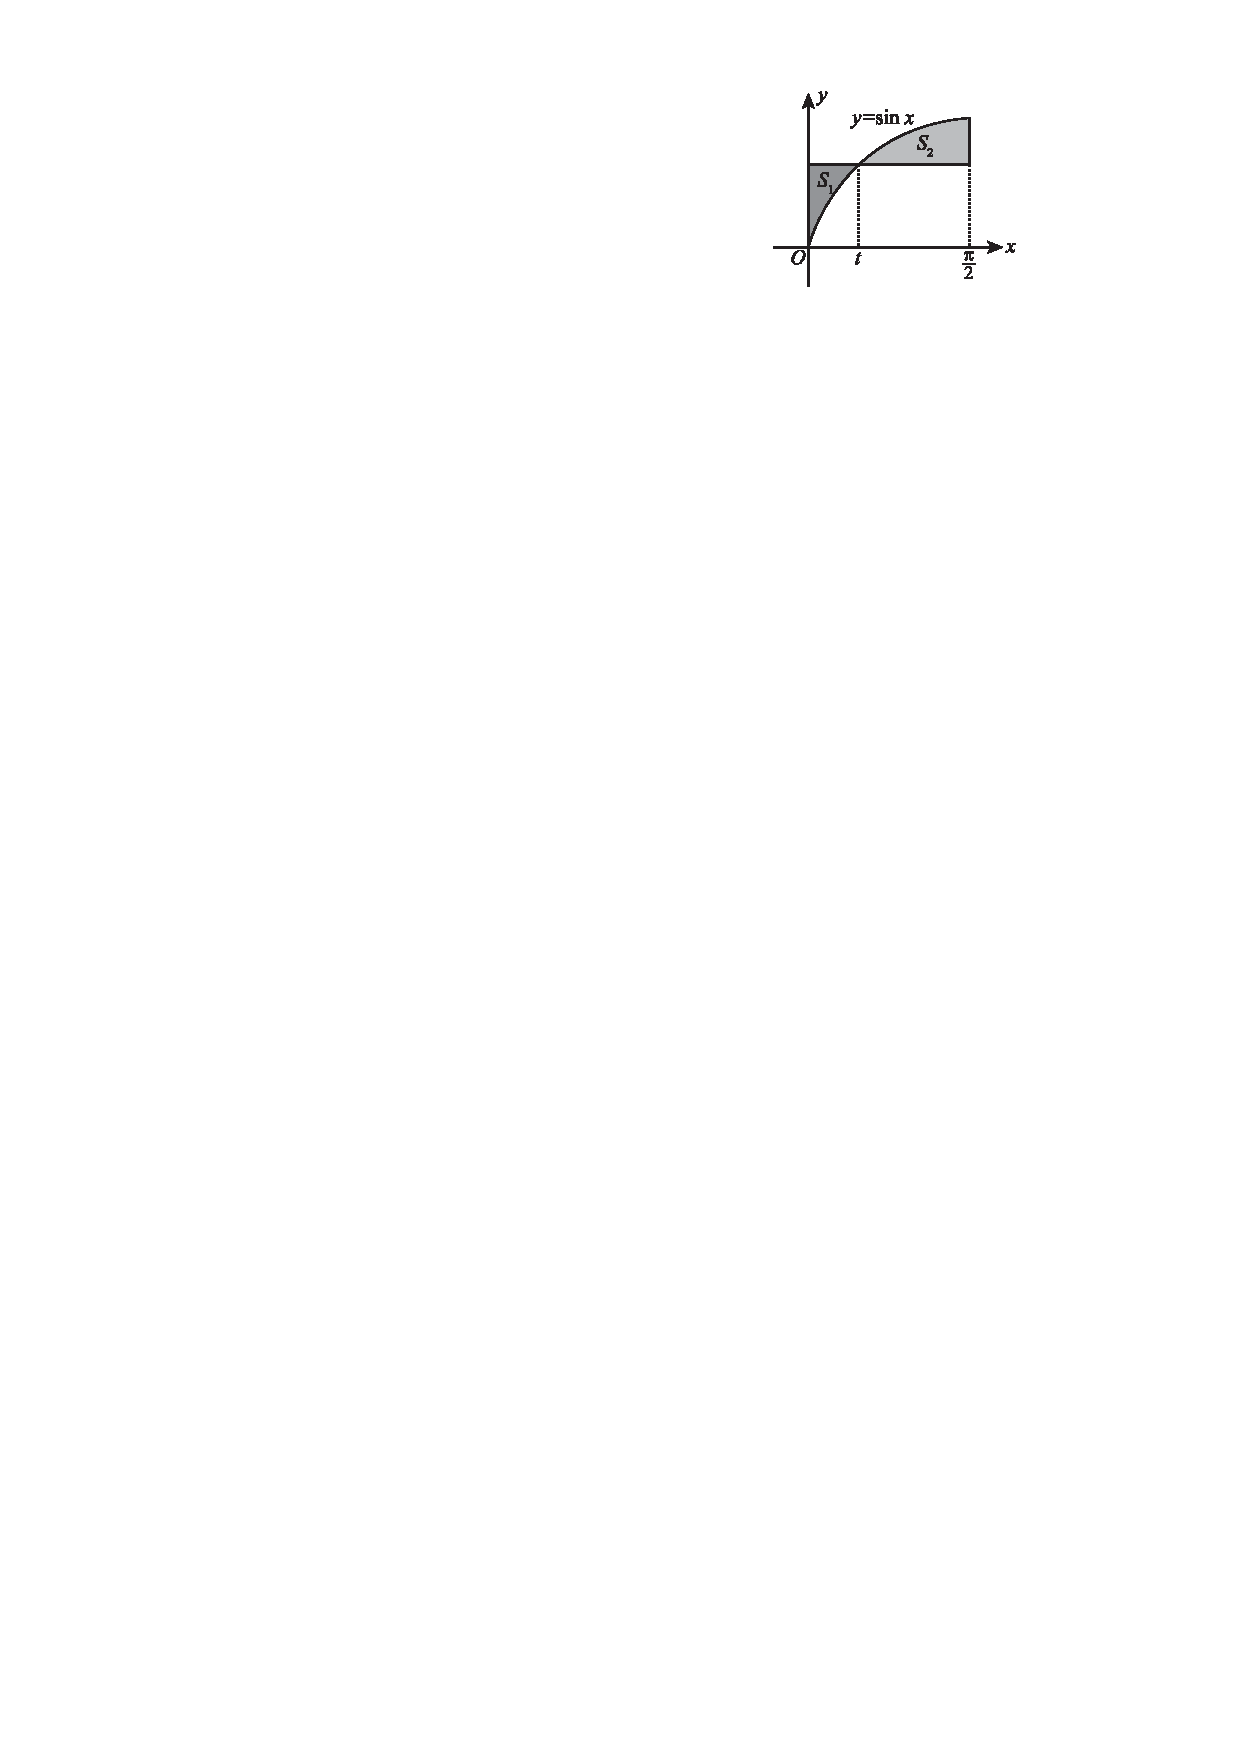
\includegraphics[width=.48\linewidth]{../assets/figures/page-011-04.pdf}\end{center}

\subsection*{五、（本题满分6分）}

将函数 \(\displaystyle f(x)=\dfrac{\displaystyle 1}{\displaystyle x^2-3x+2}\) 展开成 \(\displaystyle x\) 的幂级数，并指出收敛区间。


\subsection*{六、（本题满分5分）}

计算二重积分 \(\displaystyle \iint_D e^{x^2}\,dx\,dy\)，其中 \(\displaystyle D\) 是第一象限中由直线 \(\displaystyle y=x\) 和曲线 \(\displaystyle y=x^3\) 围成的封闭区域。


\subsection*{七、（本题满分6分）}

已知某商品的需求量 \(\displaystyle x\) 对价格 \(\displaystyle p\) 的弹性 \(\displaystyle \eta=-3p^3\)，而市场对该商品的最大需求量为1（万件）。求需求函数。


\subsection*{八、（本题满分8分）}

解线性方程组


\[\fitmath{\displaystyle \begin{cases}2x_1-x_2+4x_3-3x_4=-4,\\x_1+x_3-x_4=-3,\\3x_1+x_2+x_3=1,\\7x_1+7x_3-3x_4=3.\end{cases}}\]


\subsection*{九、（本题满分7分）}

设矩阵 \(\displaystyle A\) 和 \(\displaystyle B\) 满足 \(\displaystyle AB=A+2B\)，求矩阵 \(\displaystyle B\)，其中


\[\fitmath{\displaystyle A=\begin{pmatrix}4&2&3\\1&1&0\\-1&2&3\end{pmatrix}.}\]


\subsection*{十、（本题满分6分）}

求矩阵 \(\displaystyle A\) 的特征值与对应的特征向量，其中


\[\fitmath{\displaystyle A=\begin{pmatrix}-3&-1&2\\0&-1&4\\-1&0&1\end{pmatrix}.}\]


\subsection*{十一、（本题共2小题，每小题4分，满分8分）}

（1）已知随机变量 \(\displaystyle X\) 的概率分布为 \(\displaystyle P\{X=1\}=0.2,\allowbreak \ P\{X=2\}=0.3,\allowbreak \ P\{X=3\}=0.5\)，试写出 \(\displaystyle X\) 的分布函数 \(\displaystyle F(x)\)。


（2）已知随机变量 \(\displaystyle Y\) 的概率密度为


\[\fitmath{\displaystyle f(y)=\begin{cases}\dfrac{\displaystyle y}{\displaystyle a^2}e^{-y^2/(2a^2)},&y>0,\\0,&y\le0,\end{cases}}\]


求随机变量 \(\displaystyle Z=\dfrac{\displaystyle 1}{\displaystyle Y}\) 的数学期望 \(\displaystyle E(Z)\)。


\subsection*{十二、（本题满分8分）}

假设有两箱同种零件：第一箱内装50件，其中10件一等品；第二箱内装30件，其中18件一等品。现从两箱中随意挑出一箱，然后从该箱中先后随机取两个零件（取出的零件均不放回）。试求：


（1）先取出的零件是一等品的概率 \(\displaystyle p\)；


（2）在先取出的零件是一等品的条件下，第二次取出的零件仍然是一等品的条件概率 \(\displaystyle q\)。


\subsection*{（试卷V）}

\subsection*{一、判断题（本题共5小题，每小题2分，满分10分）}

（1）【同试卷IV 第一、（1）题】


（2）【同试卷IV 第一、（2）题】


（3）若函数 \(\displaystyle f(x)\) 在区间 \(\displaystyle (a,\allowbreak b)\) 上严格单增，则对区间 \(\displaystyle (a,\allowbreak b)\) 内任何一点 \(\displaystyle x\) 有 \(\displaystyle f\prime(x)>0\)。


（4）若 \(\displaystyle A\) 为 \(\displaystyle n\) 阶方阵，\(\displaystyle k\) 为常数，且 \(\displaystyle |A|\) 和 \(\displaystyle |kA|\) 为 \(\displaystyle A\) 和 \(\displaystyle kA\) 的行列式，则 \(\displaystyle |kA|=k|A|\)。


（5）【同试卷IV 第一、（5）题】


\subsection*{二、选择题（本题共5小题，每小题2分，满分10分）}

（1）【同试卷IV 第二、（1）题】


（2）【同试卷IV 第二、（2）题】


（3）【同试卷IV 第二、（3）题】


（4）【同试卷IV 第二、（4）题】


（5）对于任意两个事件 \(\displaystyle A\) 和 \(\displaystyle B\)，有 \(\displaystyle P(A-B)=\)（　　）


（A）\(\displaystyle P(A)-P(B)\)。 （B）\(\displaystyle P(A)-P(B)+P(AB)\)。 （C）\(\displaystyle P(A)-P(AB)\)。 （D）\(\displaystyle P(A)-P(\bar B)-P(\overline{AB})\)。


\subsection*{三、计算下列各题（本题共5小题，每小题4分，满分20分）}

（1）求极限 \(\displaystyle \lim_{x\to+\infty}\dfrac{\displaystyle \ln(1+1/x)}{\displaystyle \operatorname{arccot}x}\)。


（2）【同试卷IV 第三、（2）题】


（3）【同试卷IV 第三、（3）题】


（4）计算定积分 \(\displaystyle \int_{1/2}^1 e^{\sqrt{2x-1}}\,dx\)。


（5）求不定积分 \(\displaystyle \int\dfrac{\displaystyle x\,dx}{\displaystyle x^4+2x^2+5}\)。


\subsection*{四、（本题满分10分）}

考虑函数 \(\displaystyle y=x^2,\allowbreak \ 0\le x\le1\)。问：


（1）\(\displaystyle t\) 取何值时，右图中阴影部分的面积 \(\displaystyle S_1\) 与 \(\displaystyle S_2\) 之和 \(\displaystyle S=S_1+S_2\) 最小？


（2）\(\displaystyle t\) 取何值时，面积 \(\displaystyle S=S_1+S_2\) 最大？


\begin{center}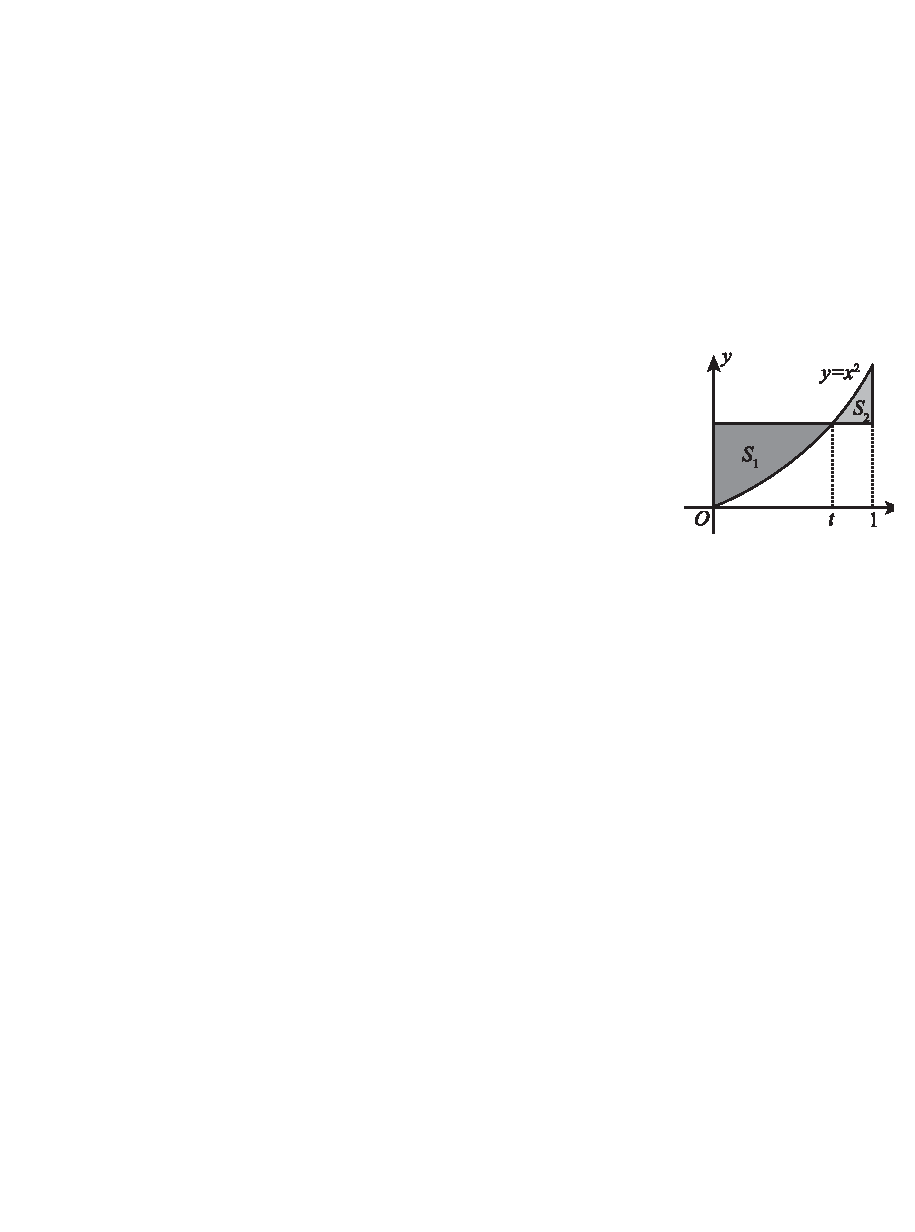
\includegraphics[width=.48\linewidth]{../assets/figures/page-021-10.pdf}\end{center}

\subsection*{五、（本题满分5分）【同试卷IV 第六题】}

\subsection*{六、（本题满分8分）}

设某产品的总成本函数为 \(\displaystyle C(x)=400+3x+\dfrac{\displaystyle 1}{\displaystyle 2}x^2\)，而需求函数为 \(\displaystyle p=\dfrac{\displaystyle 100}{\displaystyle \sqrt x}\)，其中 \(\displaystyle x\) 为产量（假定等于需求量）、\(\displaystyle p\) 为价格，试求：


（1）边际成本； （2）边际收益； （3）边际利润； （4）收益的价格弹性。


\subsection*{七、（本题满分8分）【同试卷IV 第八题】}

\subsection*{八、（本题满分7分）【同试卷IV 第九题】}

\subsection*{九、（本题满分6分）【同试卷IV 第十题】}

\subsection*{十、（本题满分8分）}

已知随机变量 \(\displaystyle X\) 的概率分布为 \(\displaystyle P\{X=1\}=0.2,\allowbreak \ P\{X=2\}=0.3,\allowbreak \ P\{X=3\}=0.5\)，试写出 \(\displaystyle X\) 的分布函数 \(\displaystyle F(x)\)，并求 \(\displaystyle X\) 的数学期望与方差。


\subsection*{十一、（本题满分8分）【同试卷IV 第十二题】}
\end{document}
